% LaTeX-Vorlage für Versuchsprotokolle
% Autor: Simon May
% Datum: 2014-08-16

% Es gibt die Dokumenttypen scrartcl ("Artikel"), scrreprt ("Bericht"),
% scrbook ("Buch") und scrlettr2 ("Brief"). Diese gehören zum KOMA-Skript,
% bieten mehr Optionen als die "Standardklassen" und sollten besonders für
% deutsche Texte benutzt werden.
% Natürlich gibt es noch weitere Klassen, z.B. beamer für Präsentationen.
\documentclass[
	ngerman,        % Sprache für z.B. Babel
	a4paper,        % Papierformat
	oneside,        % Einseitig
	%twoside,       % Zweiseitig
	%twocolumn,     % Zweispaltig
	12pt,           % Schriftgröße
	pagesize=auto,  % schreibt die Papiergröße korrekt ins Ausgabedokument
	headsepline     % Linie unter der Kopfzeile
]{scrartcl}

% --- Pakete einbinden
% --- Pakete einbinden
% --- Pakete erweitern LaTeX um zusätzliche Funktionen. Dies ist ein Satz nützlicher Pakete.

% Silbentrennung; Sprache wird durch Option bei \documentclass festgelegt
\usepackage{babel}
% Verwendung der Zeichentabelle T1 (Sonderzeichen etc.)
\usepackage[T1]{fontenc} 
% Legt die Zeichenkodierung der Eingabedatei fest, z.B. UTF8
\usepackage[utf8]{inputenc}
% Schriftart
\usepackage{lmodern}

% Einige LaTeX-Bugfixes
\usepackage{fixltx2e}
% Nutzen von +, -, *, / in \setlength u.ä. (z.B. \setlength{\a + 3cm})
\usepackage{calc}
% Wird benötigt, um \ifthenelse zu benutzen
\usepackage{xifthen}
% Optionen für eigene definierte Befehle
\usepackage{xparse}

% Verbessertes Aussehen von Text
\usepackage{microtype}
% Automatische Anführungszeichen
\usepackage[autostyle]{csquotes}
% Wird für Kopf- und Fußzeile benötigt
\usepackage{scrpage2}
% Einfaches Wechseln zwischen unterschiedlichen Zeilenabständen
\usepackage{setspace}
% Optionen für Listen (enumerate, itemize, ...)
\usepackage{enumitem}
% Zusätzliche Optionen für Tabellen (tabular)
\usepackage{array}

% Mathepaket (intlimits: Grenzen über/unter Integralzeichen)
\usepackage[intlimits]{amsmath}
% Mathe-Symbole, \mathbb etc.
\usepackage{amssymb}
% Weitere Mathebefehle
\usepackage{mathtools}
% "Schöne" Brüche im Fließtext
\usepackage{xfrac}
% Ermöglicht die Nutzung von \SI{Zahl}{Einheit} u.a.
\usepackage{siunitx}

% Farben
\usepackage{xcolor}
% Zum flexiblen Einbinden von Grafiken (\includegraphics)
\usepackage{graphicx}
% .tex-Dateien mit \includegraphics einbiden
\usepackage{gincltex}
% Abbildungen im Fließtext
\usepackage{wrapfig}
% Zitieren, Bibliographie
\usepackage[style=verbose, backend=biber]{biblatex}
% Darstellung von Captions
\usepackage[font=small, labelfont=bf, format=plain]{caption}
% Abbildungen nebeneinander
\usepackage{subcaption}
\usepackage{amsmath}

% plots
\usepackage{gnuplottex}
\usepackage{pgfplots}
%\usepgfplotslibrary{external} 
%\tikzexternalize
\pgfplotsset{compat=newest}
\pgfkeys{/pgf/number format/read comma as period}

% Genauere Position von figures
\usepackage{float}
\usepackage[section]{placeins}

% Mehrere Zeilen in table
\usepackage{multirow}

% Tables mit diagonal getrennten Zeilen
\usepackage{diagbox}

% Bessere tables
\usepackage{booktabs}

%PDF's Einbinden
\usepackage{pdfpages} 

\usepackage{rotating}

\usepackage{lscape} 

% Fussnoten in floats
\usepackage{footnote}
\makesavenoteenv{figure}

% Verlinkt Textstellen im PDF-Dokument
\usepackage[pdfpagelabels, unicode]{hyperref}
% "Schlaue" Referenzen (nach hyperref laden!)
\usepackage{cleveref}


% --- Einstellungen
% -- latex
% größere Kopfzeile (wegen LaTeX-Warnung)
\setlength{\headheight}{1.4\baselineskip}
% 1,5-facher Zeilenabstand
\onehalfspacing

% -- biblatex (Literaturverzeichnis)
\IfFileExists{res/literatur.bib}{
	\addbibresource{res/literatur.bib}
}{}

% -- csquotes
% Anführungszeichen automatisch umwandeln
\MakeOuterQuote{"}

% -- siunitx
\sisetup{
	locale=DE,
	separate-uncertainty,
	input-product=*,
	output-product=\cdot,
	quotient-mode=fraction,
	per-mode=reciprocal,
	fraction-function=\sfrac
}

% -- hyperref
\hypersetup{
	% Links/Verweise mit Kasten der Dicke 0.5pt versehen
	pdfborder={0 0 0.5}
}

% -- cleveref
\crefformat{footnote}{#2\textsuperscript{#1}#3}


% --- Eigene Befehle einbinden
% Eigene Befehle eignen sich gut, um Abkürzungen für lange Befehle zu erstellen. Die Syntax ist folgende:
% \newcommand{neuer Befahl}[Anzahl Parameter (optional)]{ein langer Befehl}
% Das folgende Beispiel fügt ein Bild mit bestimmten vorgegebenen Optionen ein:
\newcommand{\centeredImage}[1]{
	\begin{figure}[h!]
		\centering
		\includegraphics[width=0.50\textwidth]{#1}
	\end{figure}
}
% #1 ist dabei ein Parameter, den man \centeredImage übergeben muss. In 10_Titelseite.tex wird dieser Befehl verwendet. Der Parameter ist dort Bilder/titelseite.jpg.
% Benötigt man keine Parameter, dann lässt man [1] weg. Werden zusätzliche Parameter benötigt, dann kann man die Zahl auf maximal 9 erhöhen.

% Ein Befehl, um eine E-Mail-Adresse darzustellen bzw. automatisch zu verlinken
\newcommand{\email}[1]{\href{mailto:#1}{\texttt{#1}}}

% Vektoren mit Strich
\newcommand{\pvec}[1]{\vec{#1}\mkern2mu\vphantom{#1}}


% --- Variablen importieren
% Der Befehl \newcommand kann auch benutzt werden, um Variablen zu definieren:

% Nummer des Versuchs (z.B. M2):
\newcommand{\varNum}{W1}
% Name des Versuchs:
\newcommand{\varName}{Stirling-Motor}
% Datum der Durchführung:
\newcommand{\varDate}{03.06.2015}
% Autoren des Protokolls:
\newcommand{\varAutor}{Alexander Schlüter, Tobias Holthaus}
% Nummer der eigenen Gruppe:
\newcommand{\varGruppe}{Gruppe 23/mi}
% E-Mail-Adressen der Autoren:
\newcommand{\varEmail}{alx.schlueter@gmail.com,holthaus.tobias@gmail.com}
% E-Mail-Adressen anzeigen (true/false):
\newcommand{\varZeigeEmail}{true}
% Kopfzeile anzeigen (true/false):
\newcommand{\varZeigeKopfzeile}{true}
% Inhaltsverzeichnis anzeigen (true/false):
\newcommand{\varZeigeInhaltsverzeichnis}{true}
% Literaturverzeichnis anzeigen (true/false):
\newcommand{\varZeigeLiteraturverzeichnis}{true}


\newboolean{showEmail}
\setboolean{showEmail}{\varZeigeEmail}
\newboolean{showHeader}
\setboolean{showHeader}{\varZeigeKopfzeile}
\newboolean{showTOC}
\setboolean{showTOC}{\varZeigeInhaltsverzeichnis}
\newboolean{showBibliography}
\setboolean{showBibliography}{\varZeigeLiteraturverzeichnis}

\begin{document}
% Überschriften mit Serif-Schriftsatz
\addtokomafont{sectioning}{\rmfamily}
% Ändert Schriftgröße und Zeilenabstand bei Captions
\addtokomafont{caption}{\small\linespread{1}\selectfont}
% Nummerierung der Formeln entsprechend der Section (z.B. 1.1)
\numberwithin{equation}{section}

% Kopf- und Fußzeile konfigurieren
\ifthenelse{\boolean{showHeader}}{
	% Innenseite der Kopfzeile
	\ihead{\textit{\varNum\ -- \varName }}
	% Mitte der Kopfzeile
	\chead{}
	% Außenseite der Kopfzeile
	\ohead{\textit{\varAutor}}
}{
	\setheadsepline{0cm}
	\setlength{\headheight}{0cm}
	\setlength{\headsep}{0cm}
}
% Innnenseite der Fußzeile
\ifoot{}
% Mitte der Fußzeile
\cfoot{- \textit{\pagemark} -}
% Außenseite der Fußzeile
\ofoot{}

% Römische Seitenzahlen für Titelseite/Inhaltsverzeichnis
\pagenumbering{roman}

% --- Titelseite einbinden
\IfFileExists{04_Titelseite.tex}{
	% Autor: Simon May
% Datum: 2014-08-16

% Befehl, um die E-Mail-Adressen darzustellen
\makeatletter
\newcommand{\protokollemailparse}[1]{
	\@for\@tempa:=#1\do{
		\email{\@tempa}\par
	}
}
\makeatother

% Informationen für die PDF-Datei
\hypersetup{
	pdfinfo={
		Title={Versuchsprotokoll \varNum. \varName},
		Author={\varAutor}
	}
}

\begin{titlepage}
	\vspace*{2.5cm}
	\begin{center}
		\Huge
		\textbf{Versuchsprotokoll \varNum}

		\LARGE
		\varName

		\vspace{0.5cm}
		\large
		\varDate

		\IfFileExists{res/wwu_logo.png}{
			\vspace{0.5cm}
			
\includegraphics[width=0.5\textwidth]{res/wwu_logo.png}
		}{
		\vspace{4cm}
		}

		\vspace{1.5cm}
		\varAutor

		\vspace{1cm}
		\normalsize
		\varGruppe

		\ifthenelse{\boolean{showEmail}}{
			\protokollemailparse{\varEmail}
		}{}  
	\end{center}
\end{titlepage}


}{}

% --- Inhaltsverzeichnis einbinden
\ifthenelse{\boolean{showTOC}}{
	\tableofcontents
	\clearpage
}{}

% Zurücksetzen der Seitenzahlen auf arabische Ziffern
\setcounter{page}{1}
\pagenumbering{arabic}
% Ab hier mit Kopf- und Fußzeile
\pagestyle{scrheadings}

% --- Den Inhalt der Arbeit einbinden
\section{Einführung}
Eine reale Spannungsquelle wird durch das Modell des Innenwiderstandes beschrieben. Dabei wird gerechnet, als wäre ein Innenwiderstand $R_i$ in Reihe mit der eigentlichen Spannungsquelle mit Leerlaufspannung $U_0$ geschaltet. Es ergibt sich bei Belastung durch einen Außenwiderstand $R_a$ (Strom $I$):
\begin{equation}
  U_0=R_i\cdot I+R_a\cdot I
  \label{eq:innenwiderstand}
\end{equation}
Die tatsächlich gemessene Spannung an der Quelle weicht von der Leerlaufspannung ab und heißt Klemmspannung $U_{\text{Kl}}$:
\begin{equation}
  U_{\text{Kl}}=U_0-R_i\cdot I=R_a\cdot I
  \label{eq:klemmspannung}
\end{equation}
Beim Kurzschluss für $R_a=0$ fließt der endliche Strom
\begin{equation}
  I_{\text{Ks}}=U_0/R_i.
  \label{eq:kurzschluss}
\end{equation}
Die an den Verbraucher abgegebene Leistung beträgt
\begin{equation}
  P=U_0^2 \frac{R_a}{(R_a+R_i)^2}.
  \label{eq:leistung}
\end{equation}
Wir leiten die Bedingung für maximale Leistungsabgabe her:
\begin{align}
  &\frac{\mathrm{d}P}{\mathrm{d}R_a}=\frac{U_0^2}{(R_a-R_i)^2}-2\cdot \frac{R_a U_0^2}{(R_a+R_i)^3}=0 \\
  &\implies (R_a+R_i)=2R_a \implies R_a=R_i
  \label{eq:maxleistung}
\end{align}
Bei Wechselstrom wird keine konstante Spannung angelegt, sondern eine Periodisch veränderliche. In der Regel entspricht der Spannungsverlauf einer (Ko-)Sinusfunktion, jedoch sind auch andere Verläufe möglich. 
\begin{equation}
	U = U(t) = U_0 \sin(\omega t + \varphi_U)
\end{equation}
Die Stromstärke ist nur bei Ohmschen Widerständen direkt proportional zur Spannung. Bei Spule und Kondensator kommt es dagegen zu einer Phase $ \varphi = \varphi_U - \varphi_I $ zwischen Spannung und Strom.
\begin{align}
	&\text{Ohmscher Widerstand } R & U_R = R I&,~\varphi = 0 \\
	&\text{Spule mit Induktivität } L & U_L = L \frac{\di I}{\di t}&,~\varphi= \frac{\pi}{2} \\
	&\text{Kondensator mit Kapazität } C & U_C = \frac{1}{C} \int I \di t&,~\varphi = -\frac{\pi}{2}
\end{align}
Die Leistung bleibt das Produkt aus Spannung und Stromstärke. Jedoch ist meistens nur der Mittelwert von Interesse. Für Gleichstrom ergibt das
\begin{equation}
	\bar{P} = \frac{1}{T} \int_{t_0}^{t_0+T} P(t) \di t = \frac{1}{T} \int_{0}^{T} U_0 I_0 \sin^2(\omega t) \di t = \frac{U_0}{\sqrt{2}} \frac{I_0}{\sqrt{2}}
\end{equation}
Daher Definiert man die Effektivwerte 
\begin{equation}
	U_{eff} = \frac{U_0}{\sqrt{2}} \qquad\qquad I_{eff} = \frac{I_0}{\sqrt{2}}
\end{equation}
Im allgemeinen gilt
\begin{equation}
	\bar P = U_{eff}I_{eff} \cos \varphi \label{eq:phase}
\end{equation}
Um Wechselstrom zu messen sind Messgeräte oft zu träge. Dann erhält man den linearen Mittelwert
\begin{equation}
	A = \frac{1}{T} \int_{t_0}^{t_0 + T} A(t) \di t 
\end{equation}
Bei Sinuswellen ist dies $ 0 $. Daher wird stattdessen der Gleichspannungsteil, bzw. der Effektivwert verwendet 
\begin{align}
	A_= &= \frac{1}{T} \int_{t_0}^{t_0 + T} |A(t)| \di t \\
	A_{eff} &= \sqrt{\frac{1}{T} \int_{t_0}^{t_0 + T} \big(A(t)\big)^2 \di t} 
\end{align}
Bei sinusförmigen Wechselstrom ergibt sich
\begin{align}
	I_{=} &= \frac{1}{T}\int_{0}^{T}|I_{0}\sin(\omega t)| \di t=I_{0}\frac{2}{T}\int_{0}^{\frac{T}{2}}\sin(\omega t) \di t = \frac{2}{\pi} I_0 \\
	I_{eff}&=\sqrt{\frac{1}{T}\int_{0}^{T}I_{0}^{2}\sin^{2}(\omega t)\di t}=\sqrt{\frac{I_{0}^{2}}{2T}\int_{0}^{T}(1-\cos(2\omega t))\di t}=\frac{|I_{0}|}{\sqrt{2}}
\end{align}
Mit Widerständen rechnet man bei Wechselstrom mittels Scheinwiderständen. Zusammen mit der Phase lässt sich die Stromstärke in Abhängigkeit von der Zeit berechnen. Allgemein gilt
\begin{equation}
	|Z| = \frac{U_{eff}}{I_{eff}}
\end{equation} Für ohmschen Widerstand, Spule und Kondensator sind Scheinwiderstand und Phase
\begin{align}
	&\text{Ohmscher Widerstand } R & |Z|_{R} = R &,~\varphi = 0 \label{eq:Rohm} \\
	&\text{Spule mit Induktivität } L & |Z|_{L} = \omega L &,~\varphi= \frac{\pi}{2} \\
	&\text{Kondensator mit Kapazität } C & |Z|_{C} = \frac{1}{\omega C} &,~\varphi = -\frac{\pi}{2}
\end{align}
Da im Phasenraum $ Z_{R} $ senkrecht zu $ Z_{L} $ und $ Z_{C} $ ist, ist der Gesamtscheinwiderstand bei Reihenschaltung gegeben durch
\begin{equation}
	|Z| = \sqrt{|Z|_{R}^2 + (|Z|_{L} - |Z|_{C})^2}~,\qquad \tan\varphi = \frac{R_{W,L} - R_{W,C}}{R_{W,R}} \label{eq:Induk}
\end{equation}
Für den Wirkwiderstand gilt
\begin{equation}
	R_W = |Z| \cos\varphi = \frac{U_{eff}}{I_{eff}} \cos\varphi \label{eq:wirkohm}
\end{equation}
\section{Versuche}
\subsection{Aufgabe 1}
Ziel dieses Versuches ist die Bestimmung von Leerlaufspannung $U_0$ und Innenwiderstand $R_i$ von
\begin{enumerate}
  \item einer einzelnen Akkumulatorzelle
  \item drei Zellen parallel
  \item drei Zellen in Reihe.
\end{enumerate}
Dazu wird ein Stöpselwiderstand $R_a$ in Reihe und ein Spannungsmessgerät zur Messung der Klemmspannung $U_{\text{Kl}}$ parallel zu den Zellen geschaltet. Der Stöpselwiderstand fungiert als Lastwiderstand, über den der Strom $I$ reguliert werden kann. Es werden jeweils 13 Spannungswerte nach Einstellen verschiedener Widerstände $R_a$ abgenommen. Darunter sind auch Werte für den Kurzschlussfall ($R_a$=0) und für nicht geschlossenen Stromkreis ($R_a=\infty$).
\begin{table}[H]
  \centering
  \begin{tabular}{c c c} \toprule
    $R_a$ [\SI{\pm1}{\ohm}] & $U_{\text{Kl}}$ [\SI{\pm .015}{V}] & $I=U_{\text{Kl}}/R_a$ [\SI{\pm .5}{mA}] \\ \midrule
    $\infty$ & \num{1.338} & - \\
    0 & \num{0.021} & - \\
    5 & \num{0.303} & \num{60.6} \\
    10 & \num{.483} & \num{48.3} \\
    20 & \num{.717} & \num{35.8} \\
    30 & \num{.840} & \num{28.0} \\
    40 & \num{.930} & \num{23.3} \\
    50 & \num{.987} & \num{19.7} \\
    60 & \num{1.035} & \num{17.3} \\
    70 & \num{1.071} & \num{15.3} \\
    80 & \num{1.095} & \num{13.7} \\
    90 & \num{1.113} & \num{12.4} \\
    100 & \num{1.140} & \num{11.4} \\ \bottomrule
  \end{tabular}
  \caption{Messergebnis für eine Zelle}
  \label{tab:einezelle}
\end{table}

\begin{table}[H]
  \centering
  \begin{tabular}{c c c} \toprule
    $R_a$ [\SI{\pm 1}{\ohm}] & $U_{\text{Kl}}$ [\SI{\pm .05}{V}] & $I=U_{\text{Kl}}/R_a$ [\SI{\pm 1.2}{mA}] \\ \midrule
    $\infty$ & \num{4.00} & - \\
    0 & \num{0.10} & - \\
    5 & \num{0.40} & \num{80} \\
    10 & \num{.70} & \num{70} \\
    20 & \num{1.15} & \num{57.5} \\
    30 & \num{1.48} & \num{49.3} \\
    40 & \num{1.73} & \num{43.3} \\
    50 & \num{1.98} & \num{39.6} \\
    60 & \num{2.12} & \num{35.3} \\
    70 & \num{2.30} & \num{32.9} \\
    80 & \num{2.40} & \num{30.0} \\
    90 & \num{2.52} & \num{28.0} \\
    100 & \num{2.61} & \num{26.1} \\ \bottomrule
  \end{tabular}
  \caption{Messergebnis für drei Zellen parallel}
  \label{tab:einezelle}
\end{table}

\begin{table}[H]
  \centering
  \begin{tabular}{c c c} \toprule
    $R_a$ [\SI{\pm1}{\ohm}] & $U_{\text{Kl}}$ [\SI{\pm .015}{V}] & $I=U_{\text{Kl}}/R_a$ [\SI{\pm .5}{mA}] \\ \midrule
    $\infty$ & \num{1.323} & - \\
    0 & \num{0.030} & - \\
    5 & \num{0.327} & \num{65.4} \\
    10 & \num{.495} & \num{49.5} \\
    20 & \num{.717} & \num{35.9} \\
    30 & \num{.843} & \num{28.1} \\
    40 & \num{.930} & \num{23.3} \\
    50 & \num{.990} & \num{19.8} \\
    60 & \num{1.023} & \num{17.1} \\
    70 & \num{1.068} & \num{15.3} \\
    80 & \num{1.095} & \num{13.7} \\
    90 & \num{1.113} & \num{12.4} \\
    100 & \num{1.137} & \num{11.4} \\ \bottomrule
  \end{tabular}
  \caption{Messergebnis für drei Zellen in Reihe}
  \label{tab:einezelle}
\end{table}
Wir beobachten bei allen drei Messungen eine Zunahme der Klemmspannung $U_{\text{Kl}}$ und Abnahme des Stromes $I$ bei höherem Lastwiderstand $R_a$. Die Werte für eine Zelle entsprechen bis auf geringe Abweichungen den Werten für drei Zellen in Reihe. Die größte Abweichung tritt für $R_a=\SI{5}{\ohm}$ auf und beträgt $\Delta U_0=(\SI{0.327}{V}-\SI{0.303}{V})/(\SI{0.303}{V})\approx \SI{8}{\percent}$.

\subsection{Aufgabe 4}
Da es keine weiteren Angaben zur Frequenz der Wechselspannung gab, wurde von den normalen 50 Hz ausgegangen.
\begin{figure}[H] 
  \centering
	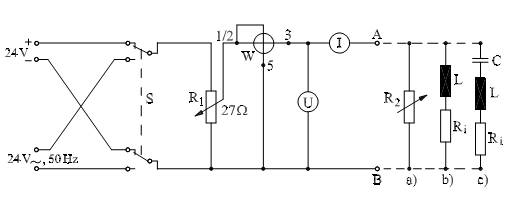
\includegraphics[width=0.7\textwidth]{Schaltplan.png}
	\caption{Schaltplan für die Aufgaben 4-8 \footcite{anleitung-ws2014}}
  \label{fig:kreisel1}
\end{figure}
In dem Aufbau wird kein Verbraucher angeschlossen um die Verlustleistung des Voltmeters zu bestimmen. Diese beträgt bei maximaler Spannung, $U_{Gleich}=27V$ oder $U_{Wechsel}=25,5V$, $P_{verlust}=1W$ und nimmt bei sinkenden Spannungen weiter ab.
\subsection{Aufgabe 5}
An den Punkten A und B wird ein ohmscher Widerstand angeschlossen, für den bei Wechsel- und Gleichspannung die möglichen Messwerte bestimmt werden.
\begin{table}[H]
  \centering
  \begin{tabular}{c | c | c | c}
    Spannungsart & Spannung U [V] $\pm0,25$ & Stromstärke I [A] $\pm 0,05$ & Leistung P [W] $\pm0,5$\\ \hline
     & 24 & 1,00 & 23,7\\
     & 20 & 0,85 & 17,0\\
     Wechselspannung & 15 & 0,68 & 9,8\\
     & 10 & 0,43 & 4,0\\
     & 5 & 0,20 & 1,0\\ \hline
     & 25 & 1,00 & 24,5\\
     & 20 & 0,82 & 16,0\\
     Gleichspannung & 15 & 0,63 & 9,0\\
     & 10 & 0,42 & 3,9\\
     & 5 & 0,20 & 0,6
  \end{tabular}
  \caption{Messwerte des ohmschen Widerstands}
  \label{tab:messungohm}
\end{table}
\begin{figure}[H]
  \centering
  \begin{tikzpicture}
    \begin{axis}[
      width=15 cm,
      height=9 cm,
      xmin=0, xmax=30,
      ymin=0, ymax=1.2,
      xlabel={Angelenkte Spannung U [V]},
      ylabel={Gemessene Stromstärke I [A]},
      legend entries={Gleichspannung, Wechselspannung, Linearer Fit beider Spannungen},
      legend pos=north west,
      domain=0.1:28,
    ]
      \addplot plot [only marks,mark=x,thick,error bars/.cd, x dir=both, x fixed=0.25, y dir=both, y fixed=0.05]  file {GleichR.txt};
      \addplot plot [only marks,mark=o,thick,error bars/.cd, x dir=both, x fixed=0.25, y dir=both, y fixed=0.05]  file {WechselR.txt};
      \addplot[mark=none] {0.04*x+0.014};
    \end{axis}
  \end{tikzpicture}
  \caption{Versuch mit ohmschen Widerstand (Spannung gegen Stromstärke)}
  \label{fig:UIOhmscher}
\end{figure}
In dem Diagramm wurde nur der Fit für Gleichspannung eingetragen, da sich dieser fast mit dem von der Wechselspannung deckt und so eine größere Übersichtlichkeit erreicht wurde.

Aufgrund des anscheinend sehr linearen Verlaufs der Messwerte für beide Spannungsarten und in Deckung mit der zu erwarteten Formel \ref{eq:Rohm} wurde mit \emph{gnuplot} nach dem \emph{least-squares}-Verfahren die Werte der beiden Spannungsarten gegen die Funktion $f(x)=m\cdot x+b$ gefittet. Ausgabe:
\begin{table}[H]
  \centering
  \begin{tabular}{c | c | c | c}
    Spannungsart & Variabel m & Variabel b & Varians der Residuals\\ \hline
    Gleichspannung & 0,04 & 0,014 & 0,00024\\
    Wechselspannung & 0,0422 & 0,007 & 0,00077
  \end{tabular}
  \caption{Linearer Fit zu Abbildung \ref{fig:UIOhmscher}}
  \label{tab:fitUIOhmscher}
\end{table}
\begin{figure}[H]
  \centering
  \begin{tikzpicture}
    \begin{axis}[
      width=15 cm,
      height=9 cm,
      xmin=0, xmax=25,
      ymin=0, ymax=30,
      xlabel={Gemessene Leistung P [W]},
      ylabel={Produkt der Stromstärke I und der Spannung U [W]},
      legend entries={Gleichspannung, Wechselspannung, Linearer Fit beider Spannungen},
      legend pos=north west,
      domain=0.1:28,
    ]
      \addplot plot [only marks,mark=x,thick,error bars/.cd, x dir=both, x fixed=0.5, y dir=both, y fixed=0.5]  file {GleichR4.txt};
      \addplot plot [only marks,mark=o,thick,error bars/.cd, x dir=both, x fixed=0.5, y dir=both, y fixed=0.5]  file {WechselR2.txt};
      \addplot[mark=none] {1.005*x+0.352};
    \end{axis}
  \end{tikzpicture}
  \caption{Versuch mit ohmschen Widerstand (Leistung gegen Produkt aus Spannung und Stromstärke)}
  \label{fig:PUIOhmscher}
\end{figure}
In dem Diagramm wurde nur der Fit für Gleichspannung eingetragen, da sich dieser fast mit dem von der Wechselspannung deckt und so eine größere Übersichtlichkeit erreicht wurde. Der Fehler des Produktes von Stromstärke und Spannung wurde nach der Gaußschen Fehlerfortpflanzung bestimmt.

Aufgrund des anscheinend linearen Verlaufs der Messwerte für beide Spannungsarten und in Deckung mit der zu erwarteten Formel \ref{eq:leistung} wurde mit \emph{gnuplot} nach dem \emph{least-squares}-Verfahren die Werte der beiden Spannungsarten gegen die Funktion $f(x)=m\cdot x+b$ gefittet. Ausgabe:
\begin{table}[H]
  \centering
  \begin{tabular}{c | c | c | c}
    Spannungsart & Variabel m & Variabel b & Varians der Residuals\\ \hline
    Gleichspannung & 1,005 & 0,352 & 0,004\\
    Wechselspannung & 1,003 & 0,164 & 0,45
  \end{tabular}
  \caption{Linearer Fit zu Abbildung \ref{fig:PUIOhmscher}}
  \label{tab:fitPUIOhmscher}
\end{table}
\subsection{Aufgabe 6}
In diesem Versuchsteil wird eine Spule an den Punkten A und B angeschlossen (Aufbau b), und für Wechselspannung die Messwerte bestimmt.
\begin{table}[H]
  \centering
  \begin{tabular}{c | c | c}
    Spannung U [V] $\pm0,25$ & Stromstärke I [A] $\pm 0,05$ & Leistung P [W] $\pm0,5$\\ \hline
    25 & 0,85 & 16,2\\
    20 & 0,67 & 10,8\\
	15 & 0,50 & 6,0\\
    10 & 0,33 & 2,5\\
    5 & 0,20 & 1,0\\ 
  \end{tabular}
  \caption{Messwerte der Spule bei Wechselspannung}
  \label{tab:messungspulewechsel}
\end{table}
\begin{figure}[H]
  \centering
  \begin{tikzpicture}
    \begin{axis}[
      width=15 cm,
      height=9 cm,
      xmin=0, xmax=30,
      ymin=0, ymax=1.2,
      xlabel={Angelenkte Spannung U [V]},
      ylabel={Gemessene Stromstärke I [A]},
      legend entries={Wechselspannung, Linearer Fit},
      legend pos=north west,
      domain=0.1:28,
    ]
      \addplot plot [only marks,mark=x,thick,error bars/.cd, x dir=both, x fixed=0.25, y dir=both, y fixed=0.05]  file {WechselL.txt};
      
      \addplot[mark=none] {0.034*x-0.0096};
    \end{axis}
  \end{tikzpicture}
  \caption{Versuch mit Spule (Spannung gegen Stromstärke)}
  \label{fig:UISpule}
\end{figure}
\begin{table}[H]
  \centering
  \begin{tabular}{c | c | c | c}
    Spannungsart & Variabel m & Variabel b & Varians der Residuals\\ \hline
    Wechselspannung & 0,034 & -0,0096 & $2,54\cdot10^{-5}$
  \end{tabular}
  \caption{Linearer Fit zu Abbildung \ref{fig:UISpule}}
  \label{tab:fitUISpule}
\end{table}
\begin{figure}[H]
  \centering
  \begin{tikzpicture}
    \begin{axis}[
      width=15 cm,
      height=9 cm,
      xmin=0, xmax=20,
      ymin=0, ymax=25,
      xlabel={Leistung P [W]},
      ylabel={Produkt der Stromstärke I und der Spannung U [W]},
      legend entries={Wechselspannung, Linearer Fit},
      legend pos=north west,
      domain=0.1:28,
    ]
      \addplot plot [only marks,mark=x,thick,error bars/.cd, x dir=both, x fixed=0.5, y dir=both, y fixed=0.5]  file {WechselL2.txt};
      
      \addplot[mark=none] {1.301*x-0.171};
    \end{axis}
  \end{tikzpicture}
  \caption{Versuch mit Spule (Leistung gegen Produkt aus Spannung und Stromstärke)}
  \label{fig:PUISpule}
\end{figure}
Der Fehler des Produktes von Stromstärke und Spannung wurde nach der Gaußschen Fehlerfortpflanzung bestimmt.
\begin{table}[H]
  \centering
  \begin{tabular}{c | c | c | c}
    Spannungsart & Variabel m & Variabel b & Varians der Residuals\\ \hline
    Wechselspannung & 1,301 & -0,171 & 0,14
  \end{tabular}
  \caption{Linearer Fit zu Abbildung \ref{fig:PUISpule}}
  \label{tab:fitPUISpule}
\end{table}
Aus dem Fit \ref{tab:fitPUISpule} ergibt sich, wenn man den $b$ Achsenabschnitt, der aus Messungenauigkeiten folgt, vernachlässigt,
\begin{equation}
U\cdot I=1,301\cdot P.
\end{equation}
Wenn man dies nun in \ref{eq:phase} einsetzt und nach dem Phasenwinkel $\varphi$ auflöst, erhält man
\begin{equation}
\varphi = \pm arccos(\frac{1}{1,301}) = \pm 39,77^\circ.
\end{equation}
Da es sich um eine Schaltung bestehend aus nur einer Spule handelt, kann man allgemein sagen, dass die Stromstärke der Spannung folgt, woraus folgt, dass gilt
\begin{equation}
\varphi = 39,77^\circ.
\end{equation}

Aus dem Fit \ref{tab:fitUISpule} ergibt sich unter der Vernachlässigung von b
\begin{equation}
I=0,034\Omega^{-1}\cdot U.
\end{equation}
Wenn man dies nun in die Formel \ref{eq:wirkohm} einsetzt erhält man
\begin{equation}
R_W=\frac{U}{I}cos(\varphi)=\frac{U}{0,034\Omega^{-1}\cdot U}cos(\varphi)=\frac{1}{0,034\Omega^{-1}}cos(\varphi)= \frac{500}{17}cos(\varphi)\Omega \approx 22,61 \Omega
\end{equation}
\subsection{Aufgabe 7}
\begin{table}[H]
  \centering
  \begin{tabular}{c | c }
    Spannung U [V] $\pm0,25$ & Stromstärke I [A] $\pm 0,05$ \\ \hline
    24,5 & 1,0 \\
    19,0 & 0,8\\
	14,0 & 0,6 \\
    9,1 & 0,4 \\
    5,0 & 0,2 \\ 
  \end{tabular}
  \caption{Messwerte der Spule bei Wechselspannung}
  \label{tab:messungspulegleich}
\end{table}
\begin{figure}[H]
  \centering
  \begin{tikzpicture}
    \begin{axis}[
      width=15 cm,
      height=9 cm,
      xmin=0, xmax=30,
      ymin=0, ymax=1.2,
      xlabel={Angelenkte Spannung U [V]},
      ylabel={Gemessene Stromstärke I [A]},
      legend entries={Gleichspannung, Linearer Fit},
      legend pos=north west,
      domain=0.1:28,
    ]
      \addplot plot [only marks,mark=x,thick,error bars/.cd, x dir=both, x fixed=0.25, y dir=both, y fixed=0.05]  file {GleichL.txt};
      
      \addplot[mark=none] {0.041*x+0.016};
    \end{axis}
  \end{tikzpicture}
  \caption{Versuch mit Spule}
  \label{fig:UIGleichSpule}
\end{figure}
\begin{table}[H]
  \centering
  \begin{tabular}{c | c | c | c}
    Spannungsart & Variabel m & Variabel b & Varians der Residuals\\ \hline
    Gleichspannung & 0,041 & 0,016 & 0,00035
  \end{tabular}
  \caption{Linearer Fit zu Abbildung \ref{fig:UIGleichSpule}}
  \label{tab:fitUIGleichSpule}
\end{table}
Aus dem Fit \ref{tab:fitUIGleichSpule} ergibt sich unter der Vernachlässigung von b
\begin{equation}
I=0,041\Omega^{-1}\cdot U.
\end{equation}
Wenn man dies nun in die Formel \ref{eq:Rohm} einsetzt erhält man
\begin{equation}
R_i=\frac{U}{I}=\frac{U}{0,041\Omega^{-1}\cdot U}=\frac{1}{0,041\Omega^{-1}}= \frac{1000}{41}\Omega = 24,\overline{39024} \Omega
\end{equation}
Aus der Formel \ref{eq:Induk} folgt
\begin{equation}
L=\sqrt{\frac{|Z|^2-R^2}{\omega^2}}\approx 0,96 H
\end{equation}
\subsection{Aufgabe 8}
\begin{figure}[H]
  \centering
  \begin{tikzpicture}
    \begin{axis}[
      width=15 cm,
      height=9 cm,
      xmin=0, xmax=30,
      ymin=0, ymax=0.65,
      xlabel={Angelenkte Spannung U [V]},
      ylabel={Gemessene Stromstärke I [A]},
      legend entries={Wechselspannung, Linearer Fit},
      legend pos=north west,
      domain=0.1:28,
    ]
      \addplot plot [only marks,mark=x,thick,error bars/.cd, x dir=both, x fixed=0.25, y dir=both, y fixed=0.05]  file {WechselLC.txt};
      
      \addplot[mark=none] {0.0229*x+0.00344};
    \end{axis}
  \end{tikzpicture}
  \caption{Versuch mit Spule und Kondensator (Spannung gegen Stromstärke)}
  \label{fig:UILC}
\end{figure}
\begin{table}[H]
  \centering
  \begin{tabular}{c | c | c | c}
    Spannungsart & Variabel m & Variabel b & Varians der Residuals\\ \hline
    Wechselspannung & 0,023 & 0,003 & $1,36\cdot10^{-5}$
  \end{tabular}
  \caption{Linearer Fit zu Abbildung \ref{fig:UILC}}
  \label{tab:fitUILC}
\end{table}
\begin{figure}[H]
  \centering
  \begin{tikzpicture}
    \begin{axis}[
      width=15 cm,
      height=9 cm,
      xmin=0, xmax=10,
      ymin=0, ymax=15,
      xlabel={Leistung P [W]},
      ylabel={Produkt der Stromstärke I und der Spannung U [W]},
      legend entries={Wechselspannung, Linearer Fit},
      legend pos=north west,
      domain=0:9,
    ]
      \addplot plot [only marks,mark=x,thick,error bars/.cd, x dir=both, x fixed=0.5, y dir=both, y fixed=0.5]  file {WechselLC2.txt};
      
      \addplot[mark=none] {1.62*x+0.27};
    \end{axis}
  \end{tikzpicture}
  \caption{Versuch mit Spule(Leistung gegen Produkt aus Spannung und Stromstärke)}
  \label{fig:PUILC}
\end{figure}
Der Fehler des Produktes von Stromstärke und Spannung wurde nach der Gaußschen Fehlerfortpflanzung bestimmt.
\begin{table}[H]
  \centering
  \begin{tabular}{c | c | c | c}
    Spannungsart & Variabel m & Variabel b & Varians der Residuals\\ \hline
    Wechselspannung & 1,62 & 0.27 & 0,038
  \end{tabular}
  \caption{Linearer Fit zu Abbildung \ref{fig:PUILC}}
  \label{tab:fitPUILC}
\end{table}
Der Phasenwinkel lässt sich analog zu Aufgabe 6 berechnen
\begin{equation}
\varphi=arccos(1,62^{-1})=51,88^{\circ}.
\end{equation}
Ebenso kann man den Widerstand |Z| so wie bei Aufgabe 6 berechnen.
\begin{equation}
|Z|=\frac{1}{0,023\Omega^{-1}}=\frac{1000}{23}\Omega\approx 43,48\Omega
\end{equation}

Damit kann nun die Kapazität des Kondensators berechnet werden
\begin{equation}
C=\frac{1}{\omega^2L+\omega\sqrt{|Z|^2-R^2}}=10,54\mu F
\end{equation}
\section{Diskussion}

\notecite{anleitung-ws2014}


% --- Anhang einbinden
\IfFileExists{20_Anhang.tex}{
	\clearpage
	\appendix
	\section{Anhang}
	\subsection{Fehlerrechnung}
\subsubsection{Magnetfeld aus Induktionsspannung}
Da Windungszahl und Fläche der Spule sowie die Frequenz des Wechselstroms als nicht Fehlerbehaftet angesehen werden, muss nur die Unsicherheit bei der Spannungsmessung berücksichtigt werden. Es gilt 
\begin{equation}
	\Delta B_{eff} = \left|\frac{\partial }{\partial U_{eff}} \frac{U_{eff}}{\omega NF} \Delta U_{eff}\right| = \left|\frac{\Delta U_{eff}}{\omega N F}\right|
\end{equation}

}{}

% --- Literaturverzeichnis mit BibLaTeX
\ifthenelse{\boolean{showBibliography}}{
	\clearpage
	\printbibliography
}{}

\end{document}

